\documentclass[xcolor={dvipsnames,table},aspectratio=169]{beamer}
\usepackage[utf8]{inputenc}
\usepackage[T1]{fontenc}
\usepackage[brazil]{babel}
\usepackage{graphics,amssymb,amsfonts,amsmath}
\usepackage{tikz}
\usepackage{enumerate,hyperref}
\usepackage{palatino}
\usepackage{ragged2e}
\usepackage{minted}
\usepackage{booktabs}
\usepackage{tabto}
\usepackage{verbatim}
\usepackage[export]{adjustbox}
\usepackage{tikz}                   
\usepackage{xcolor}
\usepackage{textcomp} % para usar \textdegree
\usetikzlibrary{shadows}
\usetheme{AnnArbor}
\usecolortheme{orchid}
\usefonttheme[onlymath]{serif}

\newminted{java}{bgcolor=cyan!10}

\newcolumntype{C}[1]{>{\centering\let\newline\\\arraybackslash\hspace{0pt}}m{#1}}

\AtBeginSection[]{
  \begin{frame}
  \vfill
  \centering
  \begin{beamercolorbox}[sep=8pt,center,shadow=true,rounded=true]{title}
    \usebeamerfont{title}\insertsectionhead\par%
  \end{beamercolorbox}
  \vfill
  \end{frame}
}

\title[\sc{Decisões}]{Decisões}
\author[Roland Teodorowitsch]{Roland Teodorowitsch}
\institute[FPROG - EP - PUCRS]{Fundamentos de Programação - Escola Politécnica - PUCRS}
\date{4 de maio de 2023}

\begin{document}
\justifying

%-------------------------------------------------------
\begin{frame}
	\titlepage
\end{frame}

%=======================================================
\section{Introdução}

%-------------------------------------------------------
\begin{frame}\frametitle{Objetivos}
\begin{itemize}
	\item Implementar decisões (simples e complexas) usando o comando \texttt{if}
	\item Comparar números e cadeias de caracteres
	\item Escrever comandos usando o tipo de dado \texttt{boolean}
\end{itemize}
\end{frame}

%-------------------------------------------------------
\begin{frame}\frametitle{Conteúdos}
\begin{itemize}
	\item O Comando \texttt{if}
	\item Comparando \emph{Strings}
	\item Múltiplas Alternativas
	\item Decisões Aninhadas
	\item Variáveis e operadores Booleanos
	\item Exercícios
	\item Tópicos Avançados
\end{itemize}
\end{frame}

%=======================================================
\section{O Comando if}

%-------------------------------------------------------
\begin{frame}\frametitle{Decisões}
\begin{itemize}
	\item Um programa de computador frequentemente necessita tomar decisões baseadas em alguma entrada ou em dados sendo processados
	\item Exemplos:
	\begin{itemize}
		\item Mostrar a mensagem ``Aprovado'', se o aluno tem nota de g1 maior ou igual a 7,0; ou a mensagem ``G2 ou Reprovado'', em caso contrário
		\item Ao subir incrementar um valor, verificar se esse valor já não extrapolou o valor máximo permitido
		\item Calcular o valor de uma multa e o número de pontos de um motorista que passa a uma certa velocidade acima do limite de uma via
		\item Calcular as raízes de uma equação do segundo grau ($ax^2 + bx + c = 0$) com delta podendo ser maior do que zero, igual a zero ou menor do que zero
		\item etc.
	\end{itemize}
	\item Para situações como estas, que exigem decisões, usa-se o comando \texttt{if}, que muitas vezes vem acompanhado de um \texttt{else}
\end{itemize}
\end{frame}

%-------------------------------------------------------
\begin{frame}[fragile]\frametitle{O Comando \texttt{if}}
\begin{itemize}
	\item \texttt{if} é o principal comando de decisão em Java
	\item Nos fluxogramas, \texttt{if} é representado por um losango
	\item O comando \texttt{if} deve especificar uma condição (expressão que gera um \texttt{boolean}) entre parênteses e um comando ou bloco para ser executado se a condição for verdadeira (\texttt{true})
\small{
\begin{javacode}
if ( delta < 0.0 )
   System.out.println("SEM raizes reais");
\end{javacode}
}
	\item \texttt{else} pode ser usado para especificar o que fazer se a condição for falsa (\texttt{false})
\small{
\begin{javacode}
if ( g1 >= 7.0 )
   System.out.println("Aprovado");
else
   System.out.println("G2 ou Reprovado");
\end{javacode}
}	
\end{itemize}
\end{frame}

%-------------------------------------------------------
\begin{frame}[fragile]\frametitle{Expressões Lógicas}
\begin{itemize}
	\item A condição ou teste do \texttt{if} é uma \textbf{expressão lógica} (	resultado \texttt{true} ou \texttt{false})
	\item Comparações entre variáveis e expressões numéricas são feitas usando \textbf{operadores relacionais}
\begin{javacode}
if (tamanhoAtual > LIMITE) {...}  // MAIO
if (tamanhoAtual >= LIMITE) {...} // MAIOR OU IGUAL
if (tamanhoAtual < LIMITE) {...}  // MENOR 
if (tamanhoAtual <= LIMITE) {...} // MENOR OU IGUAL
if (tamanhoAtual == LIMITE) {...} // IGUAL
if (tamanhoAtual != LIMITE) {...} // DIFERENTE
\end{javacode}
	\item Cálculos são feitos antes das comparações
\begin{javacode}
if ( tamanhoAtual + 1 < LIMITE )
   tamanhoAtual = tamanhoAtual + 1;
\end{javacode}
\end{itemize}
\end{frame}

%-------------------------------------------------------
\begin{frame}\frametitle{Exemplos de Expressões Lógicas}
\begin{itemize}
	\item \texttt{3 <= 4} \tabto{3cm} {\footnotesize\emph Resultado: \texttt{true}}
	\item \texttt{3 > 4} \tabto{3cm} {\footnotesize\emph Resultado: \texttt{false}}
	\item \texttt{4 < 4} \tabto{3cm} {\footnotesize\emph Resultado: \texttt{false}}
	\item \texttt{4 <= 4} \tabto{3cm} {\footnotesize\emph Resultado: \texttt{true}}
	\item \texttt{3 == 5 - 2} \tabto{3cm} {\footnotesize\emph Resultado: \texttt{true}}
	\item \texttt{3 != 5 - 1} \tabto{3cm} {\footnotesize\emph Resultado: \texttt{true}}
	\item \texttt{3 =< 4} \tabto{3cm} {\footnotesize\emph Resultado: \textbf{ERRO DE SINTAXE:} o operador correto é \texttt{<=}}
	\item \texttt{3 = 6 / 2} \tabto{3cm} {\footnotesize\emph Resultado: \textbf{ERRO DE SINTAXE:} o operador correto é \texttt{==}}
	\item \texttt{"10"} \texttt{> 5} \tabto{3cm} {\footnotesize\emph Resultado: \textbf{ERRO DE SINTAXE:} NÃO se pode comparar \emph{strings} com números}
\end{itemize}
\end{frame}

%-------------------------------------------------------
\begin{frame}\frametitle{Fluxogramas}
\begin{itemize}
	\item Já vimos alguns exemplos de fluxogramas
	\item Um fluxograma mostra a estrutura de tarefas e decisões que tem que ser executadas para resolver um problema
	\item Os elementos básicos de um fluxograma são:
\begin{figure}[h]
	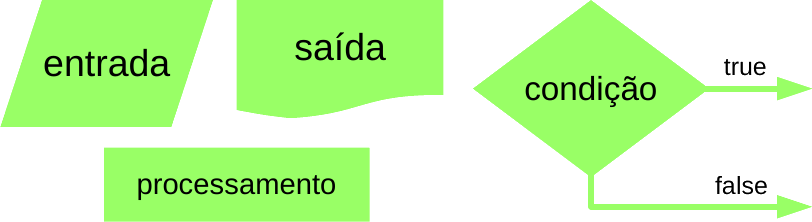
\includegraphics[height=0.25\paperheight,center]{pucrs-ep-fprog-unidade_03-decisoes-laminas-elementos_de_fluxogramas.png}
\end{figure}
	\item Os elementos de um fluxograma são conectados com setas
	\item Nunca aponte uma seta para dentro de outro ramo (isso dificulta o entendimento e a manutenção)
\end{itemize}
\end{frame}
	
%-------------------------------------------------------
\begin{frame}[fragile]\frametitle{Fluxograma do comando \texttt{if}}
\begin{itemize}
	\item Um comando \texttt{if} pode não necessitar fazer nada se a condição for falsa
\begin{columns}
\begin{column}{0.4\textwidth}
	\begin{center}
	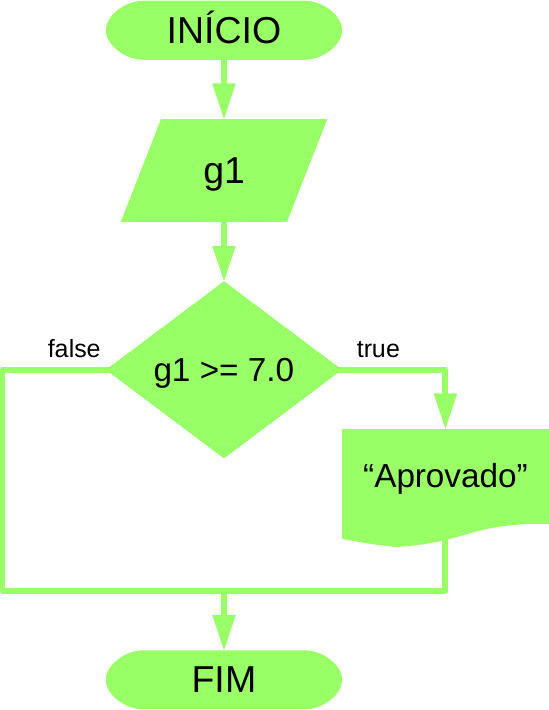
\includegraphics[height=0.6\paperheight]{pucrs-ep-fprog-unidade_03-decisoes-laminas-fluxograma_if.png}
	\end{center}
\end{column}
\begin{column}{0.6\textwidth}
	\scriptsize{\inputminted[bgcolor=cyan!10]{java}{src/Aprovado.java}}
\end{column}
\end{columns}
\end{itemize}
\end{frame}

%-------------------------------------------------------
\begin{frame}[fragile]\frametitle{Fluxograma do comando \texttt{if} com \texttt{else}}
\begin{itemize}
	\item Um comando \texttt{if} pode especificar o que fazer quando a condição for verdadeira e o que fazer quando ela for falsa (\texttt{else})
\begin{columns}
\begin{column}{0.4\textwidth}
	\begin{center}
	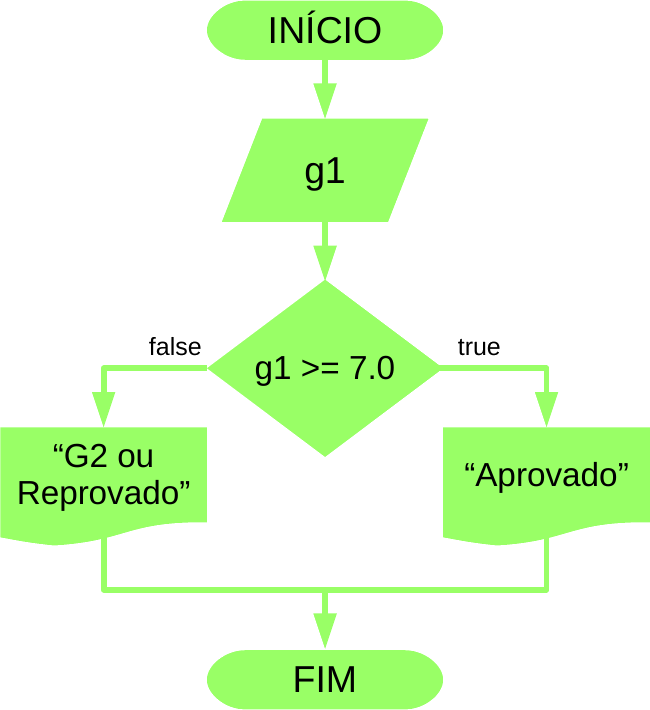
\includegraphics[height=0.6\paperheight]{pucrs-ep-fprog-unidade_03-decisoes-laminas-fluxograma_if_else.png}
	\end{center}
\end{column}
\begin{column}{0.6\textwidth}
	\tiny{\inputminted[bgcolor=cyan!10]{java}{src/AprovadoOuNao.java}}
\end{column}
\end{columns}
\end{itemize}
\end{frame}

%-------------------------------------------------------
\begin{frame}[fragile]\frametitle{Fluxograma com mais de 2 ``ramos''}
\begin{itemize}
	\item Quando há mais de duas opções pode-se usar um \texttt{if}/\texttt{else} dentro de um \texttt{if} e/ou \texttt{else}
\begin{columns}
\begin{column}{0.4\textwidth}
	\begin{center}
	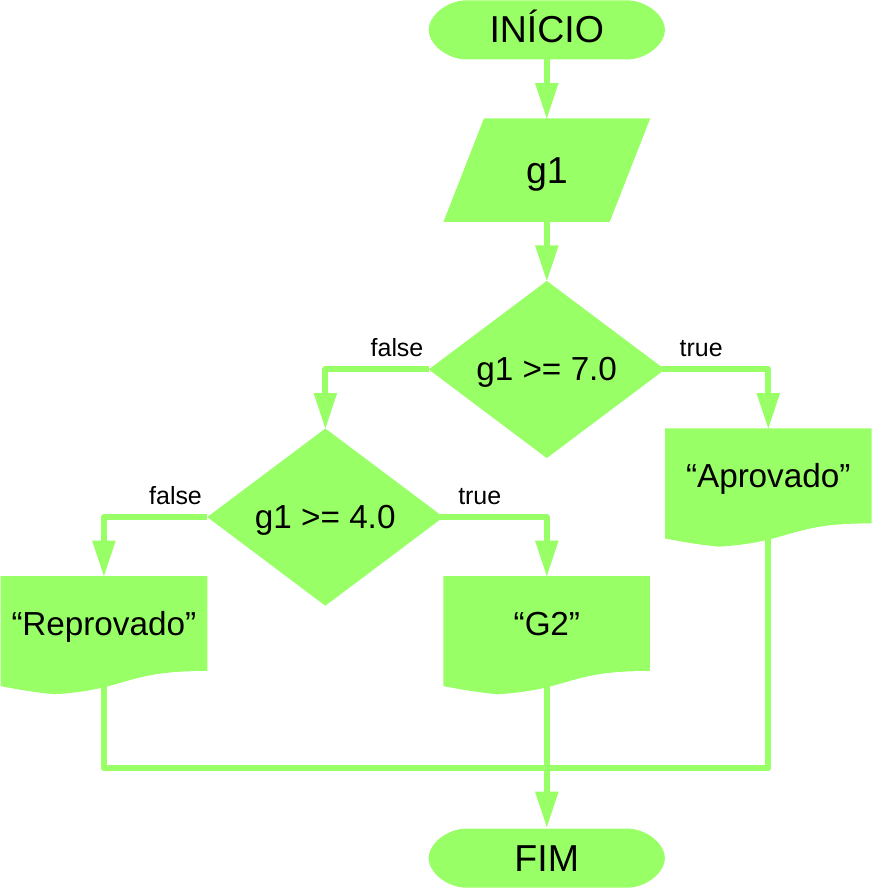
\includegraphics[height=0.6\paperheight]{pucrs-ep-fprog-unidade_03-decisoes-laminas-fluxograma_if_else_aninhado.png}
	\end{center}
\end{column}
\begin{column}{0.6\textwidth}
	\tiny{\inputminted[bgcolor=cyan!10]{java}{src/AprovadoG2OuReprovado.java}}
\end{column}
\end{columns}
\end{itemize}
\end{frame}

%-------------------------------------------------------
\begin{frame}[fragile]\frametitle{Fluxograma com mais ramos}
\begin{columns}
\begin{column}{0.4\textwidth}
	\begin{center}
	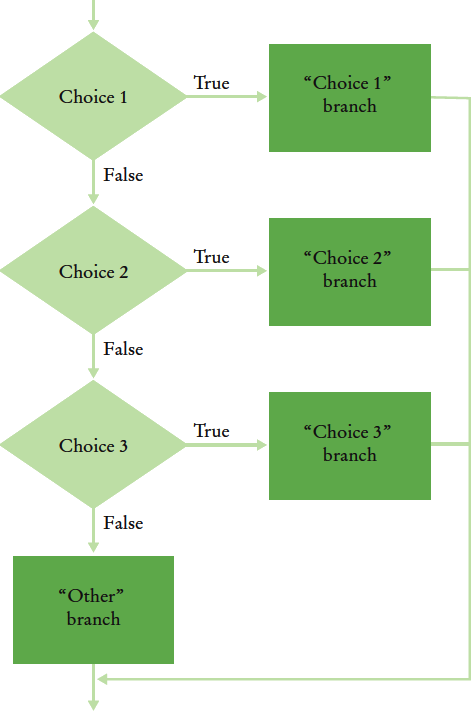
\includegraphics[height=0.7\paperheight]{pucrs-ep-fprog-unidade_03-decisoes-laminas-if_com_varios_ramos.png}
	\end{center}
\end{column}
\begin{column}{0.6\textwidth}
\scriptsize{
\begin{javacode}
if ( teste1 ) {
   System.out.println("Ramo 1");
}
else {
   if ( teste2 ) {
      System.out.println("Ramo 2");
   }
   else {
      if ( teste3 ) {
         System.out.println("Ramo 3");
      }
      else {
         System.out.println("Ramo 4");
      }	
   }
}
\end{javacode}
}
\end{column}
\end{columns}
\end{frame}

%-------------------------------------------------------
\begin{frame}[fragile]\frametitle{Dicas sobre o Uso de Chaves}
\begin{itemize}
	\item O código Java é estruturado em blocos
	\item Uma indentação consistente torna o entendimento do código muito mais fácil
	\item Dois estilos de indentação comuns são os seguintes:
	\begin{itemize}
		\item Abre-chaves embaixo do \texttt{if} e fecha-chaves na mesma coluna
\begin{javacode}
if (tamanhoAtual < LIMITE)
{
   tamanhoAtual = tamanhoAtual + 1;
}
\end{javacode}
		\item Abre-chaves na linha do \texttt{if} e fecha-chaves na mesma coluna do \texttt{if}
\begin{javacode}
if (tamanhoAtual < LIMITE) {
   tamanhoAtual ++;
}
\end{javacode}
	\end{itemize}
\end{itemize}
\end{frame}

%-------------------------------------------------------
\begin{frame}[fragile]\frametitle{Dicas sobre o Uso de Chaves}
\begin{itemize}
	\item Mesmo que para seleção de um único comando NÃO seja necessário, para quem está aprendendo, recomenda-se sempre usar chaves
	\begin{itemize}
		\item Em vez de
\begin{javacode}
if (tamanhoAtual < LIMITE)
   tamanhoAtual = tamanhoAtual + 1;
\end{javacode}
		\item Prefira usar
\begin{javacode}
if (tamanhoAtual < LIMITE) {
   tamanhoAtual = tamanhoAtual + 1;
}
\end{javacode}
	\end{itemize}
\end{itemize}
\end{frame}

%-------------------------------------------------------
\begin{frame}[fragile]\frametitle{Erros Comuns}
\begin{itemize}
	\item Um erro comum é colocar um \texttt{;} depois do comando \texttt{if}:
\begin{javacode}
if (tamanhoAtual > LIMITE) ;
{
   tamanhoAtual = tamanhoAtual + 1;
}
\end{javacode}
	\item Um \texttt{;}, sem comando antes, é um \textbf{comando vazio}
	\item Portanto, no exemplo acima, o comando \texttt{if} \textbf{NÃO FARÁ NADA} se o teste for verdadeiro (comando vazio) e o bloco (entre chaves) será executado independentemente do teste
\end{itemize}	
\end{frame}

%-------------------------------------------------------
\begin{frame}\frametitle{Exemplo}
\begin{itemize}
\item \textbf{Problema:} A livraria da Universidade realiza um Dia Kilobyte de Descontos sempre no dia 24 de outubro, dando um desconto de 8\% em todos as compras de acessórios de computador se o preço for menor do que R\$128,00, e um desconto de 16\% se o preço é no mínimo R\$128,00. Faça um programa em Java que leia o valor original das compras, calculando e mostrando o valor da compra com o desconto aplicado.
\end{itemize}
\end{frame}

%-------------------------------------------------------
\begin{frame}\frametitle{Exemplo: Passos}
\begin{itemize}
\item \textbf{Passos:}
	\begin{enumerate}
		\item Decida qual será a condição para decisão:\\ \texttt{preço original < 128?}
		\item Escreva o pseudocódigo para o ramo verdadeiro:\\ \texttt{preço com desconto = 0,92 x preço original}
		\item Escreva o pseudocódigo para o ramo falso:\\ \texttt{preço com desconto = 0,84 x preço original}
		\item Faça uma verificação dos operadores relacionais, testando-os com valores abaixo ($127$), igual ($128$) e acima ($129$)
		\item Remova a duplicação:\\ \texttt{preço com desconto = \_\_\_ x preço original}
		\item Teste ambos os ramos:\\ \texttt{preço com desconto = 0,92 x 100 = 92\\preço com desconto = 0,84 x 200 = 168}
		\item Escreva o código em Java
	\end{enumerate}
\end{itemize}
\end{frame}

%-------------------------------------------------------
\begin{frame}[fragile]\frametitle{Exemplo: Solução}
\scriptsize{\inputminted[bgcolor=cyan!10]{java}{src/Livraria.java}}
\end{frame}

%-------------------------------------------------------
\begin{frame}\frametitle{Exercícios}
\begin{enumerate}
	\item Escreva um programa em Java que verifique se um número inteiro lido do terminal é par ou ímpar.
	\item Escreva um programa em Java que verifique se um número real lido do terminal é negativo, zero  ou positivo.
	\item Implemente um programa para ler os coeficientes $a$, $b$ e $c$ de uma equação do segundo grau, calculando e mostrando as raízes reais dessa equação\\$ax^2 + bx + c = 0$. A solução pode ser obtida com a fórmula de Bhaskara
\[x=\frac{-b\pm\sqrt{\Delta}}{2a}\]
onde: $\Delta = b^2-4ac$.
\end{enumerate}
\end{frame}

%-------------------------------------------------------
\begin{frame}\frametitle{Dica sobre o Exercício 3}
\begin{itemize}
	\item Para que a equação seja do segundo grau, deve-se ter $a\neq 0$
	\item O valor de $\Delta$ determina se:
	\begin{itemize}
		\item há duas raízes reais ($\Delta > 0$)
		\item há uma raiz real ($\Delta = 0$) ou
		\item NÃO há raízes reais ($\Delta < 0$)
	\end{itemize}
	\item É importante testar essas condições no programa...
\end{itemize}
\end{frame}
	
%-------------------------------------------------------
\begin{frame}\frametitle{Solução do Exercício 1: \texttt{ParOuImpar.java}}
	\scriptsize{\inputminted[bgcolor=cyan!10]{java}{src/ParOuImpar.java}}
\end{frame}

%-------------------------------------------------------
\begin{frame}\frametitle{Solução do Exercício 2: \texttt{NegativoZeroPositivo.java}}
	\tiny{\inputminted[bgcolor=cyan!10]{java}{src/NegativoZeroPositivo.java}}
\end{frame}

%-------------------------------------------------------
\begin{frame}\frametitle{Solução do Exercício 3: \texttt{Bhaskara.java}}
	\tiny{\inputminted[bgcolor=cyan!10]{java}{src/Bhaskara.java}}
\end{frame}

%=======================================================
\section{Comparando Strings}

%-------------------------------------------------------
\begin{frame}[fragile]\frametitle{Comparando \emph{Strings}}
\begin{itemize}
	\item \emph{Strings} são um pouco ``especiais'' em Java
	\item Não use o operador \texttt{==} com \emph{strings}
	\begin{itemize}
		\item O seguinte trecho funciona, mas na verdade compara a localização de duas \emph{strings} e não os seus conteúdos
\begin{javacode}
if (string1 == string2) ...
\end{javacode}
		\item Em vez disto uso o método \texttt{equals}:
\begin{javacode}
if (string1.equals(string2)) ...
\end{javacode}
	\end{itemize}
\end{itemize}
\end{frame}

%-------------------------------------------------------
\begin{frame}[fragile]\frametitle{Exemplos}

\begin{javacode}
if ( "Tomate".substring(0,3).equals("Tom") )
   System.out.println( ">>> true <<<" );
else
   System.out.println( "false" );

if ( "Tomate".substring(0,3) == ("Tom") )
   System.out.println( "true" );
else
   System.out.println( ">>> false <<<" );
\end{javacode}
\end{frame}

%-------------------------------------------------------
\begin{frame}[fragile]\frametitle{Mais um exemplo}
\begin{itemize}
	\item Java cria uma nova variável \texttt{String} cada vez que é usado um texto entre aspas
	\item Se há uma \emph{string} que coincida exatamente com ela, Java a reusa
\footnotesize{
\begin{javacode}
String nickname = "Rob";
if (nickname == "Rob")
   System.out.println( ">>> true <<<" );
else
   System.out.println( "false" );
\end{javacode}
\begin{javacode}
String name = "Robert";
String nickname = name.substring(0,3);
if (nickname == "Rob")
   System.out.println( "true" );
else
   System.out.println( ">>> false <<<" );
\end{javacode}
}
\end{itemize}
\end{frame}

%-------------------------------------------------------
\begin{frame}\frametitle{Ordem Lexicográfica}
\begin{itemize}
	\item Para comparar \emph{strings} pela ordem de dicionário, pode-se usar \texttt{compareTo()}
	\item Considerando duas \emph{strings} \texttt{string1} e \texttt{string2}:
	\begin{itemize}
		\item \texttt{string1.compareTo(string2)} será \textbf{menor do que zero} se \texttt{string1} vier antes de \texttt{string2}
		\item \texttt{string1.compareTo(string2)} será \textbf{igual a zero} se elas forem iguais
		\item \texttt{string1.compareTo(string2)} será \textbf{maior do que zero} se \texttt{string1} vier depois de \texttt{string2}
	\end{itemize}
	\item Observações:
	\begin{itemize}
		\item Todas as letras maiúsculas vem antes das minúsculas
		\item ``Espaço'' vem antes de todos os caracteres imprimíveis
		\item Dígitos (0-9) vem antes das letras
	\end{itemize}
	\item Lembre-se: para comparar desconsiderando a diferença entre minúsculas e maiúsculas, pode-se usar \texttt{equalsIgnoreCase} e \texttt{compareToIgnoreCase}
\end{itemize}
\end{frame}

%-------------------------------------------------------
\begin{frame}\frametitle{Exercícios}
\begin{enumerate}
{\small
	\item Escreva um programa em Java que pergunte ao usuário se ele deseja sair do programa ou não (``Sair do programa (SIM ou NÃO)? ''). Se o usuário desejar sair, execute \texttt{Sytem.exit(0);} para abandonar o programa. Em caso contrário, leia um nome completo e imprima uma saudação juntamente com o nome lido (por exemplo, se nome lido for ``Han Solo'', imprima ``Bom dia, Han Solo!''). Para testar a resposta da pergunta, seu programa deverá aceitar todas as combinações de maiúsculas e minúsculas para ``sim'', com ou sem espaços antes ou depois (por exemplo, ``Sim'', ``  sIm '', ``siM '', etc.).\\
	\item Escreva um programa em Java que leia duas palavras e verifique se elas são iguais entre si ou NÃO. Seu programa deverá imprimir uma das seguintes mensagens: ``IGUAIS'' ou ``DIFERENTES''.\\
	\item Escreva um programa em Java que leia dois nomes de pessoas e mostre esses em ordem alfabética crescente, ignornando o uso de minúsculas ou maiúsculas. Por exemplo, se forem lidos, respectivamente, ``LUKE SKYWALKER'' e ''Leia Organa'', seu programa deverá imprimir: ''Leia Organa'' e ``LUKE SKYWALKER''.\\
}
\end{enumerate}
\end{frame}

%-------------------------------------------------------
\begin{frame}\frametitle{Solução do Exercício 1: \texttt{SairDoPrograma.java}}
	\scriptsize{\inputminted[bgcolor=cyan!10]{java}{src/SairDoPrograma.java}}
\end{frame}

%-------------------------------------------------------
\begin{frame}\frametitle{Solução do Exercício 2: \texttt{IguaisOuDiferentes.java}}
	\scriptsize{\inputminted[bgcolor=cyan!10]{java}{src/IguaisOuDiferentes.java}}
\end{frame}

%-------------------------------------------------------
\begin{frame}\frametitle{Solução do Exercício 3: \texttt{OrdenaDoisNomes.java}}
	\scriptsize{\inputminted[bgcolor=cyan!10]{java}{src/OrdenaDoisNomes.java}}
\end{frame}

%=======================================================
\section{Múltiplas Alternativas}

%-------------------------------------------------------
\begin{frame}\frametitle{Múltiplas Alternativas}
\begin{itemize}
	\item Um \texttt{if} tem 2 ramos, mas o que acontece se forem necessários mais do que dois ramos?
	\item Por exemplo, uma escala para o efeito de um terremoto:
	\begin{itemize}
		\item 8 (ou mais): a maioria das edificações cai
		\item 7 até 7.99: muitas edificações destruídas
		\item 6 até 6.99: muitas edificações bastante danificadas, algumas desmoronadas
		\item 4.5 até 5.99: danos a edificações mal construídas
		\item menos do que 4.5: nenhuma edificação destruída
	\end{itemize}
\end{itemize}
\end{frame}

%-------------------------------------------------------
\begin{frame}\frametitle{Fluxograma para Múltiplos Ramos}
\begin{figure}[h]
	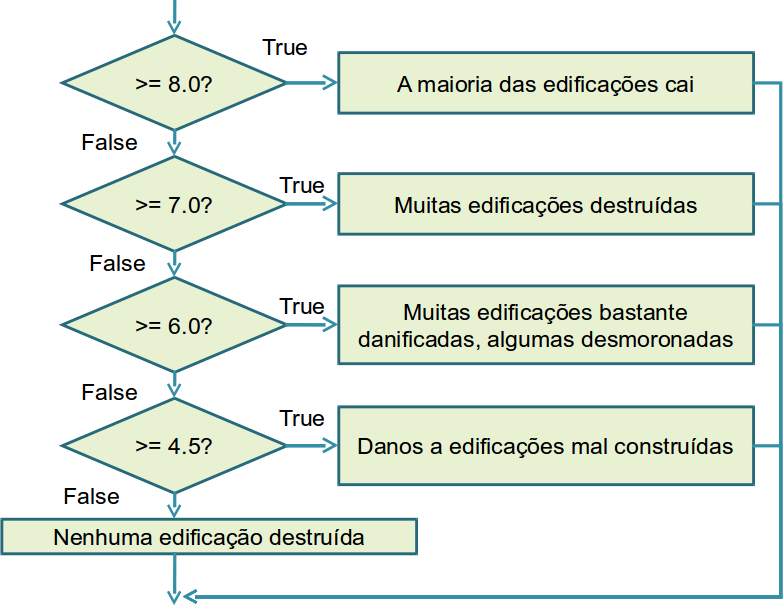
\includegraphics[height=0.7\paperheight,center]{pucrs-ep-fprog-unidade_03-decisoes-laminas-fluxograma_multiplos_ramos.png}
\end{figure}
\end{frame}

%-------------------------------------------------------
\begin{frame}[fragile]\frametitle{O que há de errado com este código?}
{\footnotesize
\begin{javacode}
if (richter >= 8.0) {
  System.out.println("A maioria das edificacoes cai");
}
if (richter >= 7.0) {
  System.out.println("Muitas edificacoes destruidas");
}
if (richter >= 6.0) {
  System.out.println("Muitas edificacoes bastante danificadas, "+
                     "algumas desmoronadas");
}
if (richter >= 4.5) {
  System.out.println("Danos a edificacoes mal construidas");
}
if (richter < 4.5) {
  System.out.println("Nenhuma edificacao destruida");
}
\end{javacode}
}
\end{frame}

%-------------------------------------------------------
\begin{frame}[fragile]\frametitle{E com este código? O que há de errado?}
{\footnotesize
\begin{javacode}
if (richter >= 8.0) {
   System.out.println("A maioria das edificacoes cai");
}
if (richter < 8.0 && richter >= 7.0) {
   System.out.println("Muitas edificacoes destruidas");
}
if (richter < 7.0 && richter >= 6.0) {
   System.out.println("Muitas edificacoes bastante danificadas, "+
                      "algumas desmoronadas");
}
if (richter < 6.0 && richter >= 4.5) {
   System.out.println("Danos a edificacoes mal construidas");
}
if (richter < 4.5) {
   System.out.println("Nenhuma edificacao destruida");
}
\end{javacode}
}
\end{frame}

%-------------------------------------------------------
\begin{frame}[fragile]\frametitle{Construção \texttt{if-else-if}}
{\footnotesize
\begin{javacode}
if (richter >= 8.0) {
   System.out.println("A maioria das edificacoes cai");
}
else if (richter >= 7.0) {
   System.out.println("Muitas edificacoes destruidas");
}
else if (richter >= 6.0) {
   System.out.println("Muitas edificacoes bastante danificadas, "+
                      "algumas desmoronadas");
}
else if (richter >= 4.5) {
   System.out.println("Danos a edificacoes mal construidas");
}
else {
   System.out.println("Nenhuma edificacao destruida");
}
\end{javacode}
}
\end{frame}

%-------------------------------------------------------
\begin{frame}\frametitle{Outra forma de Implementar Múltiplos Ramos}
\begin{itemize}
	\item O comando \texttt{switch} escolhe uma opção de um conjunto de opções
	\item Cada opção deve ser especificada por um \texttt{case}
	\item \texttt{default} trata todas as opções não especificadas em \emph{\texttt{case}s}
	\item NÃO serve para intervalos, apenas para valores discretos e para os seguintes tipos:
	\begin{itemize}
		\item tipos primitivos \texttt{byte}, \texttt{short}, \texttt{int}, \texttt{long} e \texttt{char}
		\item variáveis/objetos de classes (\texttt{Byte}, \texttt{Short}, \texttt{Integer}, \texttt{Long} e \texttt{Character}) que podem ser convertidas para os tipos primitivos suportados
		\item variáveis/objetos da classe \texttt{String}
		\item enumerações
	\end{itemize}
	\item Para encerrar um \texttt{case} deve-se usar o comando \texttt{break}
\end{itemize}
\end{frame}

%-------------------------------------------------------
\begin{frame}[fragile]\frametitle{Exemplo de \texttt{switch}/\texttt{case}}
{\small
\begin{javacode}
Scanner in = new Scanner(System.in);
int unidade = in.nextInt() % 10;
switch (unidade) {
  case 1:  System.out.println("um");     break;
  case 2:  System.out.println("dois");   break;
  case 3:  System.out.println("três");   break;
  case 4:  System.out.println("quatro"); break;
  case 5:  System.out.println("cinco");  break;
  case 6:  System.out.println("seis");   break;
  case 7:  System.out.println("sete");   break;
  case 8:  System.out.println("oito");   break;
  case 9:  System.out.println("nove");   break;
  default: System.out.println("zero");
}
\end{javacode}
}
\end{frame}

%-------------------------------------------------------
\begin{frame}[fragile]\frametitle{Enumerações}
\begin{itemize}
	\item Definem uma lista finita de valores que uma variável pode armazenar
	\item Funcionam como uma declaração de novos tipos, com uma lista de possíveis valores
{\scriptsize
\begin{javacode}
public enum EstadoCivil { 
  SOLTEIRO, CASADO, SEPARADO, DIVORCIADO, VIUVO
}
\end{javacode}
}
	\item Você pode ter qualquer número de valores, mas tem que incluir eles todos na declaração \texttt{enum}
	\item É possível declarar variáveis do tipo de uma ``enumeração''
{\scriptsize
\begin{javacode}
EstadoCivil estado = EstadoCivil.SOLTEIRO;
\end{javacode}
}
	\item Você também pode usar o operador de comparação entre eles:
{\scriptsize
\begin{javacode}
if (estado == EstadoCivil.SOLTEIRO) ... 
\end{javacode}
}
\end{itemize}
\end{frame}

%-------------------------------------------------------
\begin{frame}[fragile]\frametitle{Enumerações: Exemplos}

\begin{javacode}
public enum DiasDaSemana { 
  DOMINGO, SEGUNDA_FEIRA, TERCA_FEIRA, QUARTA_FEIRA,
  QUINTA_FEIRA, SEXTA_FEIRA, SABADO
}

public enum MesesDoAno {
  JANEIRO, FEVEREIRO, MARCO, ABRIL, MAIO, JUNHO,
  JULHO, AGOSTO, SETEMBRO, OUTUBRO, NOVEMBRO, DEZEMBRO
}

public enum EstadoSemaforo {
  VERMELHO, AMARELO, VERDE
}
\end{javacode}
\end{frame}

%-------------------------------------------------------
\begin{frame}\frametitle{Exercícios}
\begin{enumerate}
{\footnotesize
	\item Faça um programa em Java para ler o peso em Kg de um ou uma atleta adulto de Judô, mostrando a categoria à qual o ou a atleta pertence.\\
	\begin{itemize}
{\scriptsize
		\item Categorias Masculinas: Superligeiro (até 55 Kg), Ligeiro (até 60 Kg); Meio-leve (até 66 Kg), Leve (até 73 Kg), Meio-médio (até 81 Kg), Médio (até 90 Kg), Meio-pesado (até 100 Kg), Pesado (mais de 100 Kg).\\
		\item Categorias Femininas: Superligeiro (até 44 Kg), Ligeiro (até 48 Kg), Meio-leve (até 52 Kg), Leve 1
(até 57 Kg), Meio-médio (até 63 Kg), Médio (até 70 Kg), Meio-pesado (até 78 Kg), Pesado (mais de 78 Kg).\\
}
	\end{itemize}
	\item Escreva um programa em Java que leia o nome do mês, aceitando qualquer combinação de maiúsculas e minúsculas (eliminando também eventuais espaços no início e no final da leitura), e converta este nome no número inteiro de mês correspondente. Por exemplo, ``janeiro'' corresponde a 1, ``fevereiro'' corresponde a 2, etc. Nomes inválidos de mês correspondem a -1. Inicialmente implemente usando \texttt{if}/\texttt{else}, depois faça uma versão com \texttt{switch}/\texttt{case}.\\
	\item Escreva um programa em Java que leia um valor inteiro correspondendo ao dia da semana (1 correspondendo a domingo, 2 correspondendo a segunda-feira, 3 correspondendo a terça-feira, 4 correspondendo a quarta-feira, 5 correspondendo a quinta-feira, 6 correspondendo a sexta-feira e 7 correspondendo a sabado). E imprima `DIA ÚTIL'' para os dias de segunda-feira até sexta-feira, ``DESCANSO'' para sábado e domingo e ``INVÁLIDO'' para qualquer outro valor. Inicialmente implemente usando \texttt{if}/\texttt{else}, depois faça uma versão com \texttt{switch}/\texttt{case}.\\
}
\end{enumerate}
\end{frame}

%-------------------------------------------------------
\begin{frame}\frametitle{Solução do Exercício 1: \texttt{JudoMasculino.java}}
	\scriptsize{\inputminted[bgcolor=cyan!10]{java}{src/JudoMasculino.java}}
\end{frame}

%-------------------------------------------------------
\begin{frame}\frametitle{Solução do Exercício 1: \texttt{JudoFeminino.java}}
	\scriptsize{\inputminted[bgcolor=cyan!10]{java}{src/JudoFeminino.java}}
\end{frame}

%-------------------------------------------------------
\begin{frame}\frametitle{Solução do Exercício 2: \texttt{Meses.java}}
	\tiny{\inputminted[bgcolor=cyan!10]{java}{src/Meses.java}}
\end{frame}

%-------------------------------------------------------
\begin{frame}\frametitle{Solução do Exercício 2: \texttt{MesesComSwitch.java}}
	\tiny{\inputminted[bgcolor=cyan!10]{java}{src/MesesComSwitch.java}}
\end{frame}

%-------------------------------------------------------
\begin{frame}\frametitle{Solução do Exercício 3: \texttt{DiasDaSemana.java}}
	\scriptsize{\inputminted[bgcolor=cyan!10]{java}{src/DiasDaSemana.java}}
\end{frame}

%-------------------------------------------------------
\begin{frame}\frametitle{Solução do Exercício 3: \texttt{DiasDaSemanaComSwitch.java}}
	\tiny{\inputminted[bgcolor=cyan!10]{java}{src/DiasDaSemanaComSwitch.java}}
\end{frame}

%=======================================================
\section{Decisões Aninhadas}

%-------------------------------------------------------
\begin{frame}\frametitle{Decisões Aninhadas}
\begin{itemize}
	\item Você pode aninhar um \texttt{if} dentro de um ramo de um comando \texttt{if}
	\item Um exemplo simples: pedidos de bebidas em um bar
	\begin{itemize}
		\item Pergunte ao cliente o que ele quer beber
		\item Se o cliente pedir vinho:
		\begin{itemize}
			\item Peça a identidade do cliente
			\item Se a idade do cliente for maior ou igual a 21, então\\Sirva vinho
			\item Senão\\Polidamente explique como funciona a lei ao cliente 
		\end{itemize}
		\item Senão
		\begin{itemize}
			\item Sirva uma bebida não alcoólica ao cliente
		\end{itemize}
	\end{itemize}
\end{itemize}
\end{frame}

%-------------------------------------------------------
\begin{frame}\frametitle{Fluxograma de um \texttt{if} aninhado}
\begin{figure}[h]
	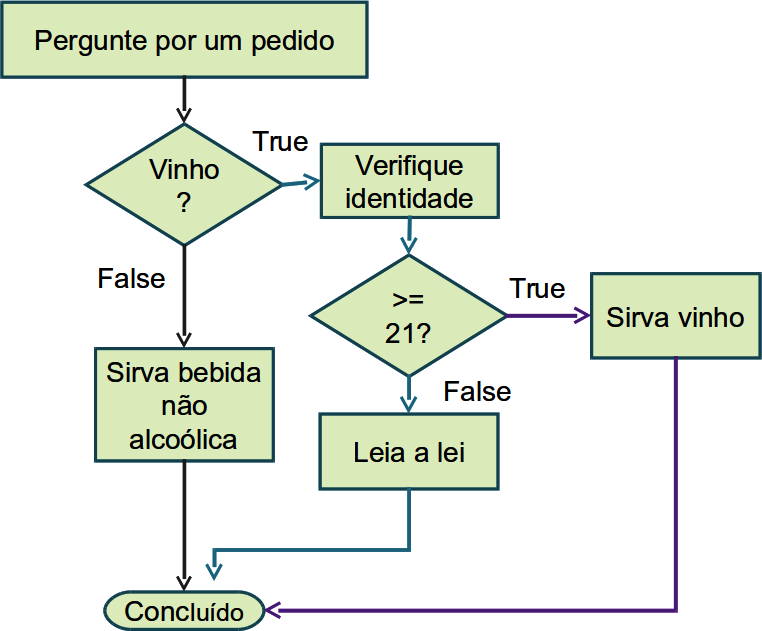
\includegraphics[height=0.65\paperheight,center]{pucrs-ep-fprog-unidade_03-decisoes-laminas-fluxograma_bebida.png}
\end{figure}
\begin{center}
{\tiny \texttt{if-else} aninhado dentro do ramo verdadeiro de um comando \texttt{if}: 3 partes}
\end{center}
\end{frame}

%-------------------------------------------------------
\begin{frame}[fragile]\frametitle{Erro Comum: \texttt{else} ``desamparado''}
\begin{itemize}
	\item Quando um \texttt{if} é aninhado dentro de outro \texttt{if}, o seguinte pode ocorrer:
\begin{javacode}
double custoDeEnvio = 5.00;
if (pais.equals("EUA"))
   if (alaskaOuHawaii.equals("SIM"))
      custoDeEnvio = 10.00;
else // Cuidado!
   custoDeEnvio = 20.00;
\end{javacode}
	\item O nível de indentação sugere que o \texttt{else} esteja relacionado ao \texttt{if} de \texttt{pais.equals("EUA")}
	\item Porém a cláusula \texttt{else} sempre se associa ao \texttt{if} mais próximo
\end{itemize}
\end{frame}

%=======================================================
\section{Variáveis e operadores Booleanos}

%-------------------------------------------------------
\begin{frame}[fragile]\frametitle{Variáveis e operadores Booleanos}
\begin{itemize}
	\item Variáveis Booleanas
	\begin{itemize}
		\item Uma variável booleana é frequentemente chamada de \emph{flag} porque pode assumir ou o valor verdadeiro (\emph{true}) ou falso (\emph{false})
		\item Java dispõe do tipo \texttt{boolean} para variáveis booleanas, que podem assumir ou \texttt{true} ou \texttt{false}
\begin{javacode}
boolean acertou = true;
boolean sair = false;
\end{javacode}
	\end{itemize}
	\item Operadores Booleanos: \texttt{\&\&} e \texttt{||}
	\begin{itemize}
		\item São usados para combinar múltiplas condições
		\item \texttt{\&\&} é o operador AND (E)
		\item \texttt{||} é o operador OR (OU)
	\end{itemize}
\end{itemize}
\end{frame}

%-------------------------------------------------------
\begin{frame}[fragile]\frametitle{Condições Combinadas: \texttt{\&\&}}
\begin{itemize}
	\item A combinação de dois testes ou condições é usada frequentemente para verificar se um valor está dentro de um intervalo
	\item Ambos os lados do AND devem ser verdadeiros para que o resultado também seja:
{\scriptsize
\begin{javacode}
if (temperatura > 0 && temperatura < 100) {
   System.out.println("Líquido"); 
}
\end{javacode}
}
\end{itemize}
\begin{figure}[h]
	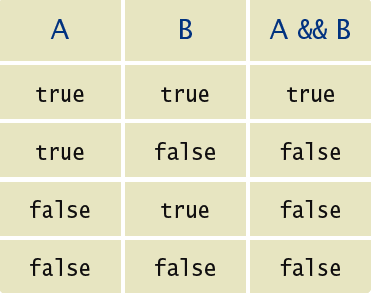
\includegraphics[height=0.35\paperheight,center]{pucrs-ep-fprog-unidade_03-decisoes-laminas-and.png}
\end{figure}
\end{frame}

%-------------------------------------------------------
\begin{frame}[fragile]\frametitle{Condições Combinadas: \texttt{||}}
\begin{itemize}
	\item Se apenas um dos testes precisa ser verdadeiro, pode-se combinar os testes com OR
	\item Se um dos lados do OR for verdadeiro, o resultado também será:
{\scriptsize
\begin{javacode}
if (saldo > 100.0 || credito > 100.0) {
   System.out.println("Aceito"); 
}
\end{javacode}
}
\end{itemize}
\begin{figure}[h]
	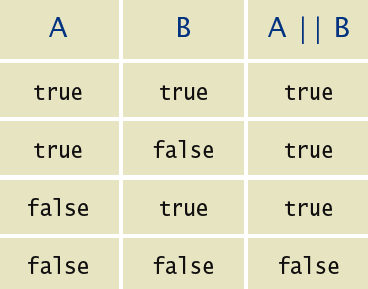
\includegraphics[height=0.35\paperheight,center]{pucrs-ep-fprog-unidade_03-decisoes-laminas-or.png}
\end{figure}
\end{frame}

%-------------------------------------------------------
\begin{frame}[fragile]\frametitle{O Operador NOT: \texttt{!}}
\begin{itemize}
	\item Se for necessário inverter o valor de uma variável booleana ou de uma condição, basta precedê-la com \texttt{!}:
\begin{figure}[h]
	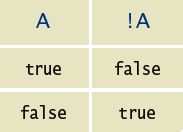
\includegraphics[height=0.15\paperheight,center]{pucrs-ep-fprog-unidade_03-decisoes-laminas-not.png}
\end{figure}
	\item O que é melhor?
\begin{columns}
\begin{column}{0.5\linewidth}
{\footnotesize
\begin{javacode}
if (!temPresencas || nota < 7.0)
   System.out.println("Desistiu?"); 
\end{javacode}
}
\end{column}
\begin{column}{0.5\linewidth}
{\footnotesize
\begin{javacode}
if (temPresencas && !(nota < 7.0))
   System.out.println("Aprovado");
\end{javacode}
}
\end{column}
\end{columns}
	\item Ao usar \texttt{!}, procure simplificar a lógica:
{\footnotesize
\begin{javacode}
if (temPresencas && nota >= 7.0)
   System.out.println("Aprovado");
\end{javacode}
}
\end{itemize}
\end{frame}

%-------------------------------------------------------
\begin{frame}[fragile]\frametitle{Fluxograma para AND}
\begin{itemize}
	\item Isto é frequentemente chamado de ``verificação de limite'', sendo usado para validar se uma entrada está entre 2 valores
\begin{javacode}
if (temperatura > 0 && temperatura < 100) {
  System.out.println("Líquido"); 
}
\end{javacode}
\end{itemize}
\end{frame}

%-------------------------------------------------------
\begin{frame}[fragile]\frametitle{Fluxograma para AND}
\begin{figure}[h]
	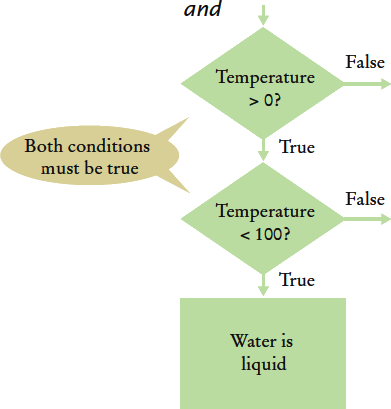
\includegraphics[height=0.70\paperheight,center]{pucrs-ep-fprog-unidade_03-decisoes-laminas-fluxograma_and.png}
\end{figure}
\end{frame}

%-------------------------------------------------------
\begin{frame}[fragile]\frametitle{Fluxograma para OR}
\begin{itemize}
	\item Outra forma de ``verificação de limite'': verifica se o valor está fora do limite
\begin{javacode}
if (temperatura <= 0 || temperatura >= 100) {
  System.out.println("Gelo ou Vapor"); 
}
\end{javacode}
\end{itemize}
\end{frame}

%-------------------------------------------------------
\begin{frame}[fragile]\frametitle{Fluxograma para OR}
\begin{figure}[h]
	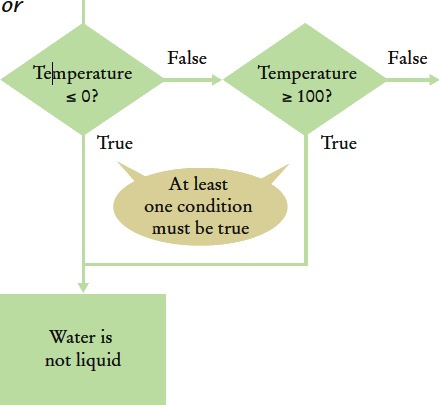
\includegraphics[height=0.70\paperheight,center]{pucrs-ep-fprog-unidade_03-decisoes-laminas-fluxograma_or.png}
\end{figure}
\end{frame}

%-------------------------------------------------------
\begin{frame}\frametitle{Exemplos de Uso de Operadores Booleanos}
{\small
\begin{center}
\begin{tikzpicture}
\node[drop shadow,fill=white,inner sep=0pt] 
{\rowcolors{1}{RoyalBlue!20}{RoyalBlue!5}
  \begin{tabular}{|p{5cm}|p{1.5cm}|p{7.5cm}|}
\hline
    \textbf{Expressão} & \textbf{Valor} & \textbf{Comentário}\\
\hline
    \texttt{0 < 200 \&\& 200 < 100}       & \texttt{false}    & Apenas a primeira condição é verdadeira\\
    \texttt{0 < 200 || 200 < 100}       & \texttt{true}     & A primeira condição é verdadeira\\
    \texttt{0 < 200 || 100 < 200}       & \texttt{true}     & Ambas as condições são verdadeiras\\
    \texttt{!(0 < 200)}       & \texttt{false}     & \texttt{0 < 200} é verdadeiro, e a sua negação é falsa\\
    \texttt{true || true \&\& false}       & \texttt{true} & \texttt{\&\&} tem maior precedência que \texttt{||}\\
    \texttt{true || (true \&\& false)}       & \texttt{true} & Os parênteses confirmam a precedência\\
    \texttt{(true || true) \&\& false}       & \texttt{false}	 & Os parênteses alteram a precedência\\
    \texttt{frozen == true}       & \texttt{frozen}     & NÃO é necessário comparar uma variável booleana com \texttt{true}\\
    \texttt{frozen == false}       & \texttt{!frozen}     & É mais claro usar \texttt{!} do que comparar com \texttt{false}	\\
\hline
  \end{tabular}
};
\end{tikzpicture}
\end{center}
}
\end{frame}

%-------------------------------------------------------
\begin{frame}[fragile]\frametitle{Erros Comuns}
\begin{itemize}
{\small
	\item O seguinte formato é usado na matemática, mas NÃO em Java:\\
\begin{javacode}
if (0 <= temperatura <= 100)  // Erro de sintaxe!
\end{javacode}
São necessárias duas comparações:\\
\begin{javacode}
if (0 <= temperatura && temperatura <= 100) 
\end{javacode}
	\item Isto também não é permitido em Java:\\
\begin{javacode}
if (input == 1 || 2)  // Erro de sintaxe!
\end{javacode}
É preciso usar 2 comparações:\\
\begin{javacode}
if (input == 1 || input == 2)
\end{javacode}
	\item Cuidado para NÃO confundir \texttt{\&\&} (dentro do intervalo) e \texttt{||} (fora do intervalo)
}
\end{itemize}
\end{frame}

%=======================================================
\section{Exercícios}

%-------------------------------------------------------
\begin{frame}\frametitle{Exercícios (1)}
\begin{enumerate}
	\item Tendo como dados de entrada a altura (em metros) e o gênero de uma pessoa, construa um programa em Java que calcule o seu peso ideal, utilizando as seguintes fórmulas:
	\begin{itemize}
		\item Para mulheres: (62.1 * altura) - 44.7
		\item Para homens: (72.7 * altura) - 58
	\end{itemize}
	\item Escreva um programa em Java que leia dois valores reais, \texttt{x} e \texttt{y}, que correspondem às coordenadas de um ponto no plano cartesiano. E imprima em que quadrante este ponto se encontra (``Quadrante 1'', ``Quadrante 2'', ``Quadrante 3'', ``Quadrante 4'') ou se ele se encontra na origem (``Origem'') ou sobre um dos eixos (``Eixo X'', ``Eixo Y'').\\
	\item Escreva um programa em Java que leia o ano de nascimento de uma pessoa, calcule e mostre sua idade, e também verifique e mostre:
	\begin{itemize}
		\item se ela já deve votar (obrigatório para pessoas com idade entre 18 e 70 anos), pode votar (opcional para pessoas com idade entre 16 e 18 anos ou maior que 70 anos) ou não pode votar (impedido para pessoas com idade menor que 16 anos); e
		\item se ela tem idade para conseguir Carteira de Habilitação (18 anos ou mais).
	\end{itemize}
\end{enumerate}
\end{frame}

%-------------------------------------------------------
\begin{frame}\frametitle{Exercícios (2)}
\begin{enumerate}
	\setcounter{enumi}{3}
	\item Escreva um programa em Java que leia o código (inteiro) de um determinado produto e mostre a sua classificação. Utilize as seguintes categorias para classificar os produtos: 1 para ``Alimento não perecível''; 2, 3 ou 4 para ``Alimento perecível''; 5 ou 6 para ``Vestuário''; 7 para ``Higiene pessoal''; e qualquer outro código para ``Inválido''.
\end{enumerate}
\end{frame}

%-------------------------------------------------------
\begin{frame}\frametitle{Exercícios (3)}
\begin{enumerate}
	\setcounter{enumi}{4}
	\item Escreva um programa em Java que leia as 4 notas de um aluno de Fundamentos de Programação: $P_1$ (nota da prova 1), $P_2$ (nota da prova 2), $M_E$ (média de exercícios) e $T_F$ (nota do trabalho final). Calcule o seu grau $G_1$, mostrando-o juntamente com uma mensagen indicando se o aluno passou por média ($G_1 \ge 7$), ficou em $G_2$ ($G_1 \ge 4$ e $G_1 < 7$) ou reprovou ($G_1 < 4$). Caso o aluno tenha ficado em $G_2$, calcule qual a nota mínima que o aluno deve tirar nessa prova para obter aprovação. Considere que a média de $G_1$ é calculada com a seguinte fórmula:
\[ G_1 = \frac{P_1 + 2 \times P_2 + M_E + 2 \times T_F}{6} \]
Lembre-se que, para obter aprovação depois da realização do $G_2$, a média aritmética entre $G_1$ e $G_2$ deve ser maior ou igual a $5$.
\end{enumerate}
\end{frame}

%-------------------------------------------------------
\begin{frame}\frametitle{Exercícios (4)}
	\begin{enumerate}
	\setcounter{enumi}{5}
	\item Escreva um trecho de programa em Java para calcular o número de pontos e o valor de multas de trânsito por excesso de velocidade. Inicialmente seu programa deverá ler o limite de velocidade da via e a velocidade do veículo (medida com um radar), ambos em quilômetros por hora e sem casas decimais. Para determinar a velocidade do veículo que será considerada, aplica-se uma tolerância de 7 km/h, se a velocidade medida for menor ou igual a 100 km/h, ou de 7\%, em caso contrário. Se a velocidade considerada for menor ou igual ao limite da via, não há multa. Se a velocidade considerada exceder 50\% do limite da via, a multa será de R\$880,41 (infração gravíssima, 7 pontos). Se a velocidade considerada exceder 20\% do limite da via, a multa será de R\$195,23 (infração grave, 5 pontos). Senão a multa será de R\$130,16 (infração média, 4 pontos).
\end{enumerate}
\end{frame}

%-------------------------------------------------------
\begin{frame}[fragile]\frametitle{Solução do Exercício 1: \texttt{PesoIdeal.java}}
	\scriptsize{\inputminted[bgcolor=cyan!10]{java}{src/PesoIdeal.java}}
\end{frame}

%-------------------------------------------------------
\begin{frame}[fragile]\frametitle{Solução do Exercício 2: \texttt{Quadrante.java}}
	\tiny{\inputminted[bgcolor=cyan!10]{java}{src/Quadrante.java}}
\end{frame}

%-------------------------------------------------------
\begin{frame}[fragile]\frametitle{Solução do Exercício 3: \texttt{Idade.java}}
	\tiny{\inputminted[bgcolor=cyan!10]{java}{src/Idade.java}}
\end{frame}

%-------------------------------------------------------
\begin{frame}[fragile]\frametitle{Solução do Exercício 4: \texttt{Classificacao.java}}
	\tiny{\inputminted[bgcolor=cyan!10]{java}{src/Classificacao.java}}
\end{frame}

%-------------------------------------------------------
\begin{frame}[fragile]\frametitle{Solução do Exercício 4: \texttt{ClassificacaoComSwitch.java}}
	\tiny{\inputminted[bgcolor=cyan!10]{java}{src/ClassificacaoComSwitch.java}}
\end{frame}

%-------------------------------------------------------
\begin{frame}[fragile]\frametitle{Solução do Exercício 5: \texttt{Notas.java}}
	\scriptsize{\inputminted[bgcolor=cyan!10]{java}{src/Notas.java}}
\end{frame}

%-------------------------------------------------------
\begin{frame}[fragile]\frametitle{Solução do Exercício 6: \texttt{MultaDeTransito.java}}
	\tiny{\inputminted[bgcolor=cyan!10]{java}{src/MultaDeTransito.java}}
\end{frame}

%=======================================================
\section{Tópicos Avançados}

%-------------------------------------------------------
\begin{frame}[fragile]\frametitle{Tópicos Avançados}
\begin{itemize}
	\item Comparação de Números de Ponto-flutuante
	\item Expressões Condicionais
	\item Casos de Teste e Acompanhamento Manual
	\item Avaliação \emph{short-circuit}
	\item Lei de De Morgan
	\item Métodos para Teste de Caracteres
	\item Validação da Entrada
	\item Exemplos
\end{itemize}
\end{frame}

%-------------------------------------------------------
\begin{frame}[fragile]\frametitle{Comparação de Números de Ponto-flutuante}
\begin{itemize}
	\item Alguns números de ponto-flutuante NÃO podem ser representados em binário de forma exata, pois, na sua conversão para binário, surge uma dízima periódica que acabará sendo interrompida
	\item Com valores reais, há risco de erros de representação e de arredondamento que podem levar a resultados inesperados
{\tiny
\begin{javacode}
double umTerco = 1.0/3.0;
if ( umTerco != 0.33333333333 )
   System.out.println("Um terço NÃO é 0,33333333333");
// RESULTADO: Um terço NÃO é 0,33333333333

double valor = 4.35, total = 4.35 * 100;
int reais = (int) total;
System.out.println("reais="+reais);
// RESULTADO: reais=434

double r = Math.sqrt(2.0);
if (r*r != 2.0)
   System.out.printf("Math.sqrt(2.0)^2 == %.20f\n",r*r);
// RESULTADO: Math.sqrt(2.0)^2 == 2,00000000000000040000
\end{javacode}
}
\end{itemize}
\end{frame}

%-------------------------------------------------------
\begin{frame}[fragile]\frametitle{Comparação de Números de Ponto-flutuante: Solução}
\begin{itemize}
	\item Define-se um erro mínimo aceitável (\texttt{EPSILON}), abaixo do qual se considera que dois valores de ponto-flutuante ``sejam iguais''
	\begin{itemize}
		\item O valor absoluto da diferença entre os dois valores deve ser menor do que determinado limite
		\item Matematicamente, diz-se que x e y estão suficientemente próximos se $|x-y|<\varepsilon$
	\end{itemize}
\begin{javacode}
final double EPSILON = 1E-14;
double r = Math.sqrt(2.0);
if (Math.abs(r * r - 2.0) < EPSILON)
   System.out.printf("Math.sqrt(2.0)^2 == 2.0");
\end{javacode}
\end{itemize}
\end{frame}

%-------------------------------------------------------
\begin{frame}[fragile]\frametitle{Expressões condicionais}
\begin{itemize}
	\item O \textbf{operador ternário} (\texttt{?:}) permite inserir uma decisão em uma expressão
	\item Por exemplo, em vez de fazer:
\begin{javacode}
if ( andar < MAIOR_ANDAR )
  novoAndar =  andar  + 1;
else
  novoAndar = andar;
\end{javacode}
pode-se fazer:
\begin{javacode}
novoAndar = andar < MAIOR_ANDAR ? andar + 1 : andar;
\end{javacode}
	\item A sintaxe das expressões condicionais é a seguinte:\\
	\texttt{condição \textbf{?} expressãoParaV \textbf{:} expressãoParaF}
\end{itemize}
\end{frame}

%-------------------------------------------------------
\begin{frame}[fragile]\frametitle{Expressões condicionais: Exemplos}
\begin{javacode}
// Exemplo 1
int inteiro = in.nextInt();
System.out.println( (inteiro%2 == 0) ? "Par" : "Impar" );

// Exemplo 2
taxaDesconto = (preco < 128) ? 0.92 : 0.84;
precoComDesconto = taxaDesconto * preco;

// OU

precoComDesconto = ( (preco < 128) ? 0.92 : 0.84 ) * preco;
\end{javacode}
\end{frame}
	
%-------------------------------------------------------
\begin{frame}\frametitle{Casos de Teste e Acompanhamento Manual}
\begin{itemize}
	\item É importante prever os ramos de decisão que podem ocorrer na execução de um programa
	\item Por exemplo:
	\begin{itemize}
		\item Estado do aluno (aprovado, em G2, reprovado)
		\item No cálculo da \emph{bhaskara}: se é uma equação do segundo grau e quais os valores possíveis para delta (negativo, zero, positivo)
	\end{itemize}
	\item Deve-se criar casos de teste para:
	\begin{itemize}
		\item Cada ramo de decisão
		\item Todos os limites dos ramos de decisão (a que ramo pertence cada valor que corresponde ao limite?...)
		\item Entradas inválidas
	\end{itemize}
\end{itemize}
\end{frame}

%-------------------------------------------------------
\begin{frame}\frametitle{Acompanhamento Manual (ou Teste de Mesa)}
\begin{itemize}
	\item Acompanhar a execução manualmente ajuda a entender se o programa está funcionando corretamente ou não
	\item Crie uma tabela com as variáveis mais importantes
	\begin{itemize}
		\item Use lápis e papel para acompanhar os valores destas variáveis
	\end{itemize}
	\item Pode ser feito com pseudocódigo ou até mesmo código Java
	\begin{itemize}
		\item Você pode marcar a execução no código com um \emph{clips}
	\end{itemize}
	\item Use valores de entrada:
	\begin{itemize}
		\item Para os quais você já sabe os resultados que serão produzidos
		\item Que testem todos os ramos possíveis do seu código 
	\end{itemize}
\end{itemize}
\end{frame}

%-------------------------------------------------------
\begin{frame}[fragile]\frametitle{Avaliação \emph{short-circuit}: \texttt{\&\&}}
\begin{itemize}
	\item Condições combinadas são avaliadas da esquerda para a direita
	\item No caso do E-lógico (\emph{and}), se uma das condições avaliadas for falsa, por que continuar avaliando as demais?
\begin{javacode}
if ( temperatura > 0 && temperatura < 100 ) {
   System.out.println("A água está líquida."); 
}
\end{javacode}
	\item Um exemplo útil:
\begin{javacode}
if ( quantidade > 0 && preco / quantidade < 10.0)
\end{javacode}
\end{itemize}
\end{frame}

%-------------------------------------------------------
\begin{frame}\frametitle{Avaliação \emph{short-circuit}: \texttt{\&\&}}
\begin{figure}[h]
	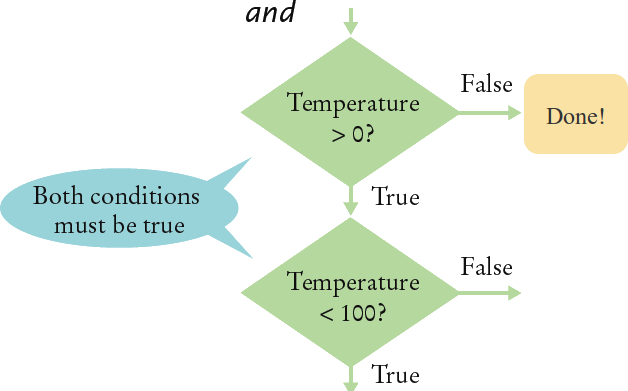
\includegraphics[height=0.70\paperheight,center]{pucrs-ep-fprog-unidade_03-decisoes-laminas-short_and.png}
\end{figure}
\end{frame}

%-------------------------------------------------------
\begin{frame}[fragile]\frametitle{Avaliação \emph{short-circuit}: \texttt{||}}
\begin{itemize}
	\item No caso do OU-lógico (\emph{or}), se alguma condição à esquerda for verdadeira, por que continuar avaliando as demais?
\begin{javacode}
if ( temperatura <= 0 || temperatura >= 100 ) {
   System.out.println("A água NÃO está líquida."); 
}
\end{javacode}
\end{itemize}
\end{frame}

%-------------------------------------------------------
\begin{frame}\frametitle{Avaliação \emph{short-circuit}: \texttt{||}}
\begin{figure}[h]
	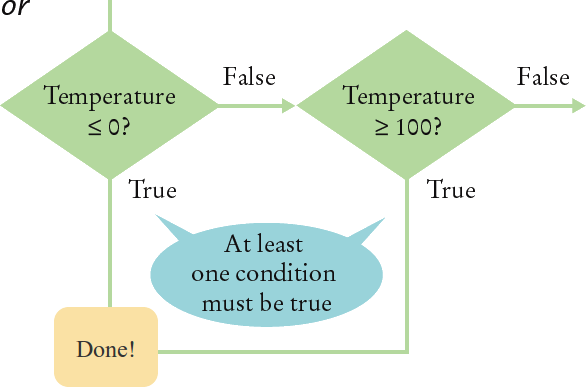
\includegraphics[height=0.70\paperheight,center]{pucrs-ep-fprog-unidade_03-decisoes-laminas-short_or.png}
\end{figure}
\end{frame}

%-------------------------------------------------------
\begin{frame}[fragile]\frametitle{Lei de De Morgan}
\begin{itemize}
	\item A Lei de De Morgan diz como negar condições \texttt{\&\&} e \texttt{||}
	\begin{itemize}
		\item \texttt{!(A \&\& B)} é o mesmo que \texttt{!A || !B}
		\item \texttt{!(A || B)} é o mesmo que \texttt{!A \&\& !B}
	\end{itemize}
	\item Exemplo: Envio para AK e HI é mais caro
{\scriptsize
\begin{javacode}
if ( !(pais.equals("USA") && !estado.equals("AK") && !estado.equals("HI")) )
   custoDeEnvio = 20.00;
\end{javacode}
\begin{javacode}
if ( !pais.equals("USA") || estado.equals("AK") || estado.equals("HI") )
   custoDeEnvio = 20.00;
\end{javacode}
}
	\item Para simplificar condições com negações de condições AND ou OR, geralmente é uma boa ideia aplicar a Lei de De Morgan para mover as negações para o nível mais interno.
\end{itemize}
\end{frame}

%-------------------------------------------------------
\begin{frame}[fragile]\frametitle{Métodos para Teste de Caracteres}
\begin{itemize}
	\item A classe \texttt{Character} tem muitos métodos para teste de caracteres
\begin{center}
\begin{tikzpicture}
\node[drop shadow,fill=white,inner sep=0pt] 
{\rowcolors{1}{RoyalBlue!20}{RoyalBlue!5}
  \begin{tabular}{|c|c|}
\hline
    \textbf{Método} & \textbf{Exemplos de Caracteres Aceitos} \\
\hline
    \texttt{isDigit}  & 0, 1, 2\\
    \texttt{isLetter}  & A, B, C, a, b, c\\
    \texttt{isLetterOrDigit}  & A, a, B, b, 0, 1\\
    \texttt{isUpperCase}  & A, B, C\\
    \texttt{isLowerCase}  & a, b, c\\
    \texttt{isWhiteSpace}  & espaço, nova linha, tabulação\\
    etc. & ...\\
\hline
  \end{tabular}
};
\end{tikzpicture}
\end{center}
	\item Pode-se usar, por exemplo:\\
{\small
\begin{javacode}
if (Character.isDigit(ch)) {
 	  System.out.printf("%c é um dígito.\n", ch);
}
\end{javacode}
}
\end{itemize}

\end{frame}

%-------------------------------------------------------
\begin{frame}[fragile]\frametitle{Validação da Entrada}
\begin{itemize}
	\item Aceitar entrada do usuário é perigoso
	\item O que acontece quando se usa \texttt{nextInt()} para ler valores inteiros e o usuário fornece uma palavra ou valor inválido?
	\item O método \texttt{hasNextInt()} da classe \texttt{Scanner} pode ajudar nesse caso
	\begin{itemize}
		\item \texttt{hasNextInt()} retorna \texttt{true} se o valor for um inteiro válido, ou \texttt{false} em caso contrário
	\end{itemize}
{\footnotesize
\begin{javacode}
if (in.hasNextInt()) {
  int inteiro = in.nextInt();
  // ... processamento do valor inteiro lido
}
else {
  System.out.println("Nenhum valor inteiro válido foi fornecido...");
}
\end{javacode}
}
	\item Há outros métodos semelhantes: \texttt{hasNextDouble()}, \texttt{hasNext()}, \texttt{hasNextLine()}, etc.
\end{itemize}
\end{frame}

%-------------------------------------------------------
\begin{frame}[fragile]\frametitle{Exemplo: \texttt{SimuladorDeElevador.java} {\tiny [Adaptado de Horstmann (2013, p. 84-85)]}}
\tiny{\inputminted[bgcolor=cyan!10]{java}{src/SimuladorDeElevador.java}}
\end{frame}

%-------------------------------------------------------
\begin{frame}[fragile]\frametitle{Exemplo: \texttt{SimuladorDeElevador2.java} {\tiny [Adaptado de Horstmann (2013, p. 117)]}}
\tiny{\inputminted[bgcolor=cyan!10]{java}{src/SimuladorDeElevador2.java}}
\end{frame}

%-------------------------------------------------------
\begin{frame}\frametitle{Exemplo: Custo de Postagem nos EUA}
\begin{itemize}
	\item O custo de envio interno nos EUA é de \$5, exceto para Hawaii e Alaska para onde o custo é de \$10. O custo internacional é de \$20.
\begin{figure}[h]
	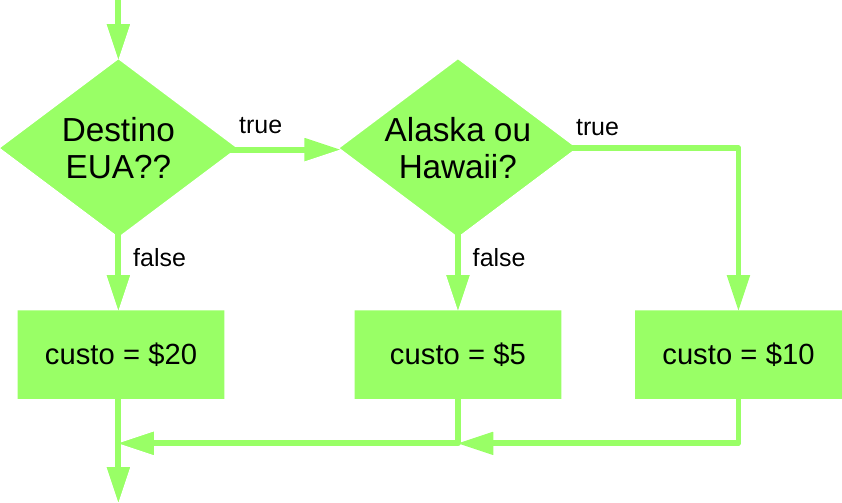
\includegraphics[height=0.50\paperheight,center]{pucrs-ep-fprog-unidade_03-decisoes-laminas-fluxograma_postagem_eua.png}
\end{figure}
\end{itemize}
\end{frame}

%-------------------------------------------------------
\begin{frame}[fragile]\frametitle{Exemplo: Custo de Postagem nos EUA}
\tiny{\inputminted[bgcolor=cyan!10]{java}{src/PostagemEUA.java}}		
\end{frame}

%-------------------------------------------------------
\begin{frame}\frametitle{Exemplo: Imposto de Renda nos EUA}
O imposto de renda anual nos EUA considera basicamente 2 alternativas iniciais: contribuição para solteiros e contribuição para casados.
Para cada uma destas possibilidades o imposto é calculado de forma diferente, conforme o ganho individual ou do casal.
\begin{itemize}
	\item Solteiro
	\begin{itemize}
		\item Renda menor ou igual a \$32.000,00\\
		taxa = 10\%
		\item Renda maior do que \$32.000,00\\
		taxa = \$3.200,00 + 25\% sobre o que exceder \$32.000,00
	\end{itemize}
	\item Casado
	\begin{itemize}
		\item Renda conjunta menor ou igual a \$64.000,00\\
		taxa = 10\%
		\item Renda conjunta maior do que \$64.000,00\\
		taxa = \$6.400,00 + 25\% sobre o que exceder \$64.000,00
	\end{itemize}
\end{itemize}
\end{frame}

%-------------------------------------------------------
\begin{frame}\frametitle{Exemplo: Imposto de Renda nos EUA}
\begin{center}
\begin{figure}[h]
	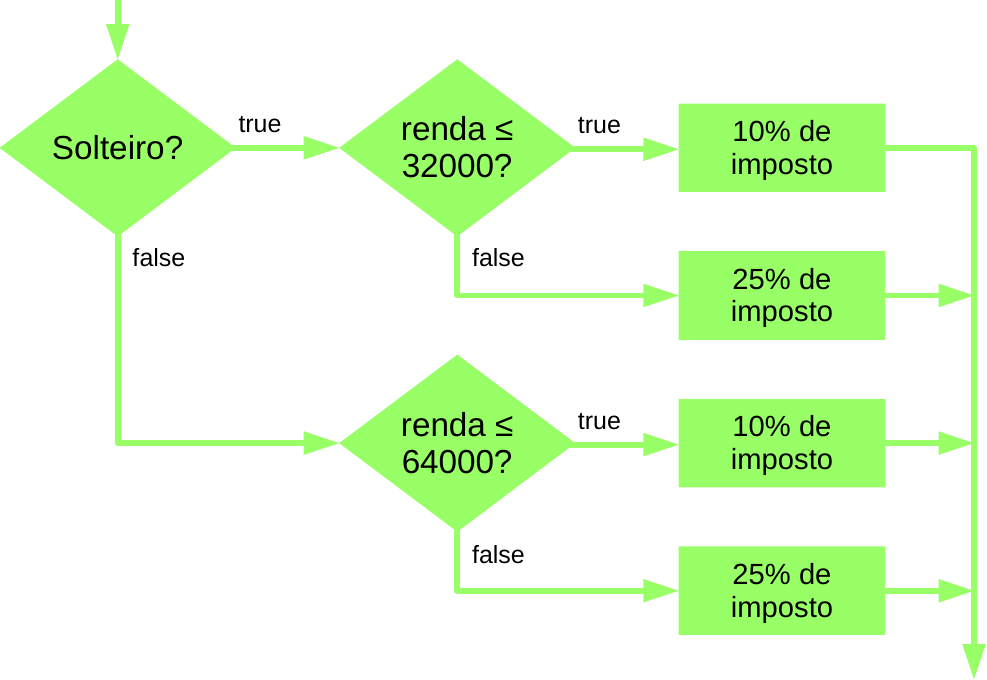
\includegraphics[height=0.65\paperheight,center]{pucrs-ep-fprog-unidade_03-decisoes-laminas-fluxograma_imposto_eua.png}
\end{figure}
\end{center}
\end{frame}

%-------------------------------------------------------
\begin{frame}[fragile]\frametitle{Exemplo: Imposto de Renda nos EUA}
\tiny{\inputminted[bgcolor=cyan!10]{java}{src/ImpostoEUA.java}}		
\end{frame}

%=======================================================
\section{Referências}

%-------------------------------------------------------
\begin{frame}\frametitle{Referências}
\noindent{HORSTMANN, C. \textbf{Java for Everyone – Late Objects}. 2. ed. Hoboken: Wiley, 2013. xxxiv, 589 p.}
\end{frame}

%=======================================================
\end{document}

